\chapter{Lecture 34 - Finite Element Method, Galerkin Method FEM in One Dimension}
\label{ch:lec34n}
\section{Objectives}
The objectives of this lecture are to:
\begin{itemize}
\item Describe a Galerkin FEM for solving a simple BVP.
\item Illustrate the method with a MATLAB implementation.
\item Demonstrate $hp$-refinement and introduce the tools required to accomplish this task.
\end{itemize}
\setcounter{lstannotation}{0}

\section{Review of the Problem}

Recall the boundary value problem that we addressed in Lecture 33:
\vspace{0.25cm}

\noindent\textbf{ODE:} $ \frac{d^2 u}{dx^2} - u = -x, \ \ 0 < x < 1$

\vspace{0.25cm}

\noindent\textbf{BCs:} $ u(0) = u(1) = 0$

\vspace{0.25cm}

\noindent\textbf{Analytic solution:} $u(x) = x - \frac{\sinh{(x)}}{\sinh{(1)}}$

\vspace{0.25cm}

\noindent The strong form of the method of weighted residuals resulted in the following problem:
\begin{align*}
\int_{0}^{1} w R \ dx &= \int_{0}^{1} w\frac{d^2u}{dx^2} \  dx - \int_{0}^{1} w u \ dx + \int_{0}^{1} wx \ dx = 0 \\
&=\int_{0}^{1} x(1-x) \left[-2a - ax(1-x) + x\right] \ dx = 0
\end{align*}
that we would solve for the unknown parameter $a$.

\vspace{0.25cm}

\noindent In order to address some technical deficiencies in the method as described in its strong form, we derived the weak form:

\vspace{0.25cm}

\begin{equation*}
w \frac{d \tilde u}{dx}\Bigl|_{0}^{1}-\int_{0}^{1}\frac{dw}{dx}\frac{d\tilde{u}}{dx} \ dx - \int_{0}^{1}w \tilde{u} \ dx + \int_{0}^{1} wx \ dx = 0
\end{equation*}
which we would solve in a similar fashion but, in this case, with a wider range of suitable trial and test functions available---in particular piece-wise linear functions would work nicely---and with the helpful presence of the boundary term in the statement which is needed for handling type-2 boundary conditions.
\vspace{0.25cm}

\noindent In this lecture we seek to describe the Finite Element Method (FEM) as a procedure by which this weak form is solved to obtain a solution that is as accurate as we would like.

\section{Galerkin Finite Element Method}

In the finite element method, in addition to converting the strong form of the governing equation into the weak form of the minimum weighted residual statement, we will discretize the domain into a finite number of elements. For example, let us consider the one-dimensional domain divided into 3 elements, using piece-wise continuous trial functions and test functions as shown in Figure \ref{fig:lec34n-discretization}.

\begin{figure}[h!]
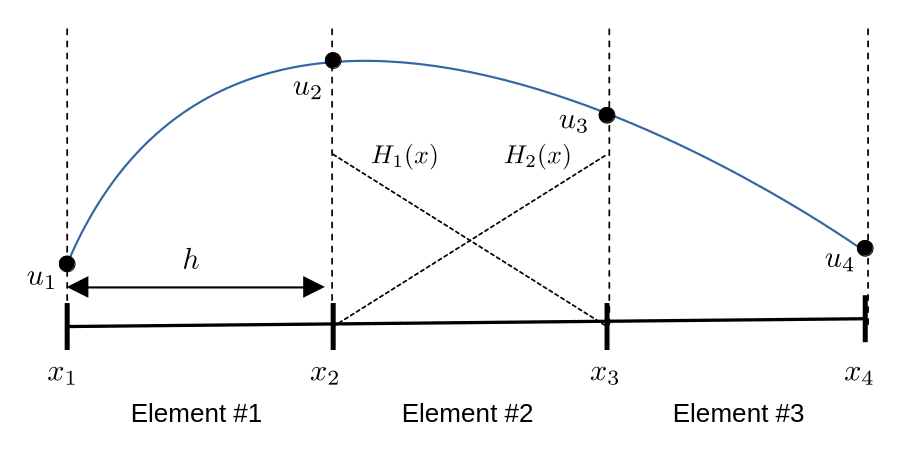
\includegraphics{lec34n-discretization.png}
\caption{Discretization of problem domain with piece-wise linear elements.}
\label{fig:lec34n-discretization}
\end{figure}
\noindent Both the trial and test functions are constructed from $H_1(x)$ and $H_2(x)$ which are commonly referred to as \emph{shape functions} that are defined on each element.\marginnote[-6.0cm]{

\noindent\textbf{Note:} The shape functions, $H_1(x)$ and $H_2(x)$, are defined on each element---i.e. $H_1(x)$ and $H_2(x)$ on element \#1 are distinct from $H_1(x)$ and $H_2(x)$ on the other elements. Nonetheless, the definitions are similar for each element, namely:

\vspace{0.1cm}

\noindent $H_1(x) = \frac{x_{i+1}-x}{h_i}, \ \ H_2(x) = \frac{x - x_i}{h_i}$
where $h_i = x_{i+1}-x_i$.

\vspace{0.25cm}

\noindent $\frac{dH_1}{dx} = -\frac{1}{h_i}, \ \ \frac{dH_2}{dx} = \frac{1}{h_i}$

\vspace{0.25cm}

\noindent Notice $H_1(x_i) = 1$ and $H_1(x_{i+1})=0$ while $H_2(x_i) = 0$ and $H_2(x_{i+1}) = 1$.  This property is referred to as \emph{cardinality} of the shape functions.  Note also that $H_1(x)+H_2(x) = 1$ if $x \in [x_i,x_{i+1}]$.  Lastly note that, in principle, the element size, $h_i$, can be different for each element.  For this example, we will take the element size to be uniform.
}

\vspace{0.25cm}

\noindent\textbf{trial functions:} $u(x) = H_1(x)u_i + H_2(x)u_{i+1}$

\vspace{0.25cm}

\noindent\textbf{test functions:} $w(x) = H_1(x) + H_2(x)$

\vspace{0.25cm}

\noindent So to recap and relate to the previous discussion about the method of minimum weighted residuals: we have a piece-wise linear trial and test functions; the unknown parameters are $\left\{u_1,u_2,u_3,u_4\right\}$; the test functions are ``the same'' as the trial functions insofar as that the are the same as the trial functions but without the unknown parameters.  Our goal is to solve for the unknown parameters, $\left\{u_1,u_2,u_3,u_4\right\}$, so that the weighted residual is minimized.

\newthought{Now we will} insert our newly defined trial functions and test functions into the weak form of the residual:\marginnote{\noindent\textbf{Note:} We have left off the boundary term.  When we eventually apply boundary conditions, we will force both the trial and test function to be equal to zero on the boundary.  Thus: $w\frac{du}{dx}\Bigl|_{0}^{1} = \cancelto{0}{w(1)}\frac{du}{dx}\Bigl|_{x=1}-\cancelto{0}{w(0)}\frac{du}{dx}\Bigl|_{x=0} = 0$.}
%\begin{fullwidth}
\begin{equation*}
-\int_{0}^{1}\frac{dw}{dx}\frac{du}{dx} \ dx - \int_{0}^{1} w u \ dx + \int_{0}^{1} wx \ dx = 0 
\end{equation*}
%\end{fullwidth}

Breaking this down one component at a time, on a per-element basis:

\begin{align*}
& \frac{dw}{dx}\frac{du}{dx} = \underbrace{\bracketVectorstack{\frac{dH_1}{dx} \\ \frac{dH_2}{dx}}}_{\sfrac{dw}{dx}} \underbrace{\bracketMatrixstack{\frac{dH_1}{dx} & \frac{dH_2}{dx}} \bracketVectorstack{u_i \\ u_{i+1}}}_{\sfrac{du}{dx}} = \bracketMatrixstack{\left(\frac{dH_1}{dx}\frac{dH_1}{dx}\right) & \left(\frac{dH_1}{dx}\frac{dH_2}{dx}\right) \\ \left(\frac{dH_2}{dx}\frac{dH_1}{dx}\right) & \left(\frac{dH_2}{dx}\frac{dH_2}{dx}\right)}\bracketVectorstack{u_i \\ u_{i+1}} = \left[K_1\right]\bracketVectorstack{u_i \\ u_{i+1}} \\
& wu = \underbrace{\bracketVectorstack{H_1 \\ H_2}}_{w}\underbrace{\bracketMatrixstack{H_1 & H_2}\bracketVectorstack{u_i \\ u_{i+1}}}_{u} = \bracketMatrixstack{\left(H_1 H_1\right) & \left(H_1 H_2\right) \\ \left(H_2 H_1\right) & \left(H_2 H_2 \right)}\bracketVectorstack{u_i \\ u_{i+1}} = \left[K_2\right]\bracketVectorstack{u_i \\ u_{i+1}} \\
& xw = \bracketMatrixstack{x_{i} & 0 \\ 0 & x_{i+1}}\bracketVectorstack{H_1 \\ H_2} = r 
\end{align*}
where, readers should bear in mind, the matrices $\left[K_1\right]$, $\left[K_2\right]$, and the vector $r$ are all functions of $x$.  Putting this all together for all 3 elements gives us:
\marginnote{
\noindent\textbf{Note:} the index $i$ corresponds to each of the 3 elements.
}
\begin{equation*}
\sum\limits_{i=1}^{3} \left[-\int_{x_i}^{x_{i+1}} \left[K_1\right]\bracketVectorstack{u_i \\ u_{i+1}} \ dx -\int_{x_i}^{x_{i+1}}\left[K_2\right]\bracketVectorstack{u_i \\ u_{i+1}} \ dx + \int_{x_i}^{x_{i+1}} r \ dx \right] = 0
\end{equation*}
We also need to deal with the integrals.  For some problems and element types, this integration can be done analytically, but the overwhelmingly common process is to carry out the integration numerically using Gauss quadrature.  For bi-linear shape functions as is used in this example, two quadrature points will be used on each element.  As always, when performing Gauss quadrature, the interval of integration needs to be mapped to $[-1,1]$ so the Gauss points are mapped accordingly and, for each element, a Jacobian is calculated and incorporated into the integration.

\begin{equation*}
\sum\limits_{i=1}^{3} \text{(Jac)}_i\left[\sum\limits_{q=1}^{qp} \text{(wgt)}_q \left\{ -\left[K_1(x_{q})+K_2(x_{q}) \right]\bracketVectorstack{u_i \\ u_{i+1}}  + r(x_{q}) \right\}  \right] = 0
\end{equation*}

\subsection{Assembly into a Linear System}
Once the quadrature has been completed, the matrices $K_1$, $K_2$ and the vector $r$ calculated on each element needs to be assembled into the system matrix.  We say ``assembly'' but this is merely the natural result of carrying out the summation of the integrals across all elements.  The output of the process is depicted in Figure \ref{fig:lec34n-system-assembly-schematic}.    
\begin{figure}[h!]
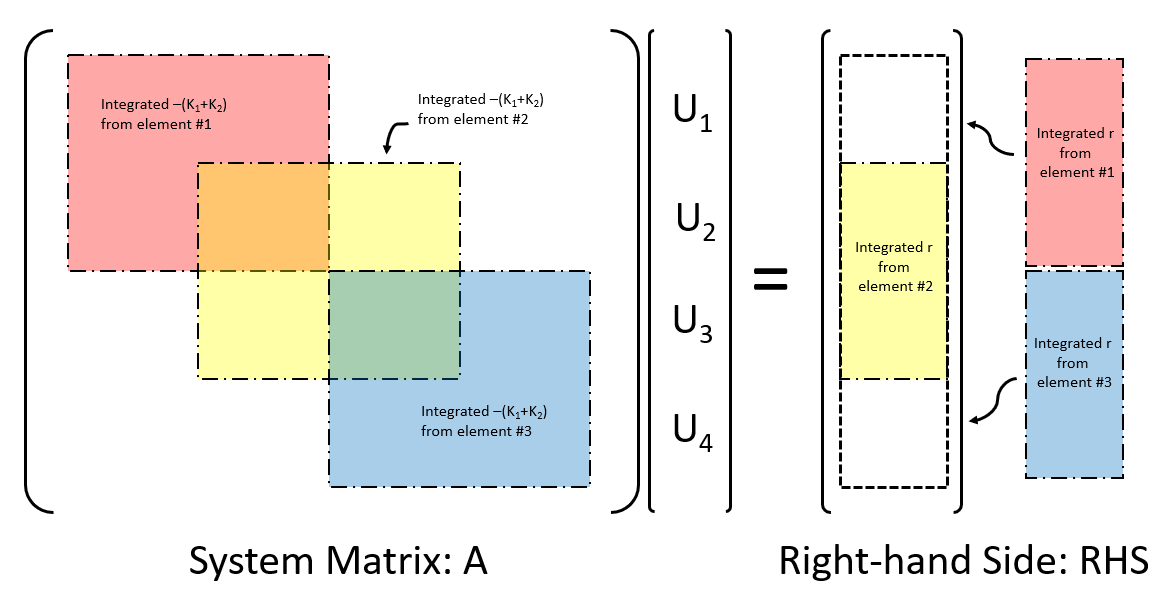
\includegraphics{lec34n-system-assembly-schematic.png}
\caption{Schematic of system assembly.}
\label{fig:lec34n-system-assembly-schematic}
\end{figure}
The matrices $K_1$ and $K_2$ of element \#1 contribute to the first two rows and columns of the system matrix; the matrices from element \#2 contribute to the second and third rows and columns; the matrices from element \#3 to the third and fourth rows and columns.  For entries where there is overlap, the results are added.  The same process is carried out for the vector $r$ that is placed on the right-hand-side.

\newthought{Once the system} matrix is assembled, all that remains is to apply the Dirichlet boundary conditions and solve by some convenient method.  The resulting coefficient values: $\left\{U_1, U_2, U_3, U_4\right\}$ are the parameters for our approximate solution.  

\section{MATLAB Implementation}

Code for an example MATLAB implementation of the Finite Element Method with linear shape functions is given below.  We start by cleaning out the workspace and initializing a representation of the exact solution.

\marginnote{

\vspace{2.0cm}

\noindent \ref{lst:ann34n-1} Always, always, always solve a known problem when learning and testing a new method.
}
\begin{lstlisting}[style=myMatlab,name=lec34n-ex1]
clear
clc
close 'all'

%% Exact Solution
u_exact = @(x) x - sinh(x)./sinh(1); /*!\annotation{lst:ann34n-1}!*/
\end{lstlisting}

\marginnote{

\vspace{2.5cm}

\noindent\ref{lst:ann34n-2} The \lstinline[style=myMatlab]{nodes} array serves as a map between global and local node numbers.  Each row contains the global node numbers of the local nodes of each element.  The column numbers correspond to the local node numbers. 

}
\begin{lstlisting}[style=myMatlab,name=lec34n-ex1]
%% Finite Element Parameters and Data Structures
a = 0; b = 1;
Ua = 0; Ub = 0; % boundary conditions

nelem = 3; % specify # of elements
gcoord = linspace(a,b,nelem+1); % x-coordinates of all nodes
nnodes = length(gcoord); %number of nodes
nodes = nan(nelem,2);   /*!\annotation{lst:ann34n-2}!*/
nodes(:,1) = 1:nelem;% x_i node number
nodes(:,2) = 2:(nelem+1);%x_i+1 node number
\end{lstlisting}
\marginnote{

\vspace{1.0cm}

\noindent\ref{lst:ann34n-3} It should seem odd that we would hard-code in the quadrature points and weights for the integration scheme.  We will soon generalize this so that the order of integration can be selected at runtime.

\vspace{0.25cm}

\noindent\ref{lst:ann34n-4} We will initialize these arrays now so they are available for the assembly process.

\vspace{0.75cm}

\noindent\ref{lst:ann34n-5} These are the elemental sub-arrays.  Alternatively, you can write your code so that these elemental values are stored directly in the system array.

\vspace{0.75cm}

\noindent\ref{lst:ann34n-6} The \lstinline[style=myMatlab]{nodes} array is used to get the coordinates of the local nodes for the current element.  This allows us to map the quadrature points to the correct physical location with each element.

\vspace{0.25cm}

\noindent\ref{lst:ann34n-7} Cell arrays are used to store the shape functions, $H(x)$, and the derivatives of shape functions, $\sfrac{dH}{dx}$, since cell arrays allow the array members to be function handles. 

\vspace{4.3cm}

\noindent\ref{lst:ann34n-8} Here we accumulate the weighted contribution from each quadrature point for the $K_1$ and $K_2$ matrices and the $r$ vector.   

}
\begin{lstlisting}[style=myMatlab,name=lec34n-ex1]
% sample points for Gauss Quadrature
q = [-0.57735027; 0.57735027];
w = [1; 1]; % weights             /*!\annotation{lst:ann34n-3}!*/
nqp = length(q); % number of quadrature points

% initialize global arrays
K1 = zeros(nnodes,nnodes);
K2 = zeros(nnodes,nnodes);   /*!\annotation{lst:ann34n-4}!*/
R = zeros(nnodes,1);

for ele = 1:nelem
    
    % local arrays to be populated
    k1 = zeros(2,2);
    k2 = zeros(2,2);       /*!\annotation{lst:ann34n-5}!*/
    r = zeros(2,1);
    
    % local mapping for GQ
    aL = gcoord(nodes(ele,1));
    bL = gcoord(nodes(ele,2));
    xT = @(t) ((bL - aL)*t + aL + bL)/2; /*!\annotation{lst:ann34n-6}!*/
    Jac = (bL - aL)/2;

    % shape functions for this element
    H = cell(2,1);         /*!\annotation{lst:ann34n-7}!*/
    hi = bL - aL;
    H{1} = @(x) (bL-x)/hi;
    H{2} = @(x) (x-aL)/hi;

    Hp = cell(2,1);
    % for generality, use functions
    Hp{1} = @(x) -1/hi;
    Hp{2} = @(x) 1/hi;

    for qp = 1:nqp        
        % sum weighted contribution at Gauss Points
        k1(1,1) = k1(1,1) + ...
            Hp{1}(xT(q(qp)))*Hp{1}(xT(q(qp)))*w(qp);
        k1(1,2) = k1(1,2) + ...
            Hp{1}(xT(q(qp)))*Hp{2}(xT(q(qp)))*w(qp);
        k1(2,1) = k1(2,1) + ...
            Hp{2}(xT(q(qp)))*Hp{1}(xT(q(qp)))*w(qp);
        k1(2,2) = k1(2,2) + ...
            Hp{2}(xT(q(qp)))*Hp{2}(xT(q(qp)))*w(qp); /*!\annotation{lst:ann34n-8}!*/
        
        k2(1,1) = k2(1,1) + ...
            H{1}(xT(q(qp)))*H{1}(xT(q(qp)))*w(qp);
        k2(1,2) = k2(1,2) + ...
            H{1}(xT(q(qp)))*H{2}(xT(q(qp)))*w(qp);
        k2(2,1) = k2(2,1) + ...
            H{2}(xT(q(qp)))*H{1}(xT(q(qp)))*w(qp);
        k2(2,2) = k2(2,2) + ...
            H{2}(xT(q(qp)))*H{2}(xT(q(qp)))*w(qp);
        
        r(1) = r(1) + xT(q(qp))*H{1}(xT(q(qp)))*w(qp);
        r(2) = r(2) + xT(q(qp))*H{2}(xT(q(qp)))*w(qp);        

    end % qp
    % apply Jacobian
    k1 = k1*Jac; k2 = k2*Jac; r = r*Jac;  /*!\annotation{lst:ann34n-9}!*/
\end{lstlisting}
\marginnote[-1.5cm]{

\vspace{1.0cm}

\noindent\ref{lst:ann34n-9} Finally the Jacobian is applied to complete the numerical quadrature.

}
\begin{lstlisting}[style=myMatlab,name=lec34n-ex1]
    % add local arrays to global arrays ("assembly")
    for i = 1:2
        for j = 1:2
            row = nodes(ele,i); col = nodes(ele,j); /*!\annotation{lst:ann34n-10}!*/
            K1(row,col) = K1(row,col) + k1(i,j);
            K2(row,col) = K2(row,col) + k2(i,j);
        end % j
        dof = nodes(ele,i);
        R(dof) = R(dof) + r(i);
    end % i
end % numel
\end{lstlisting}
\marginnote[-3.0cm]{

\vspace{0.1cm}

\noindent\ref{lst:ann34n-10} Here again the \lstinline[style=myMatlab]{nodes} array is used as a map to facilitate the global matrix assembly process.  

}
Now that the integration and assembly processes are complete to construct the system matrix, we are ready to apply the Dirichlet boundary conditions, solve for the unknown parameters, and plot the solution.  For three elements with linear shape functions, the approximate solution is shown in Figure \ref{fig:lec34n-ex1-sol}.
\begin{marginfigure}
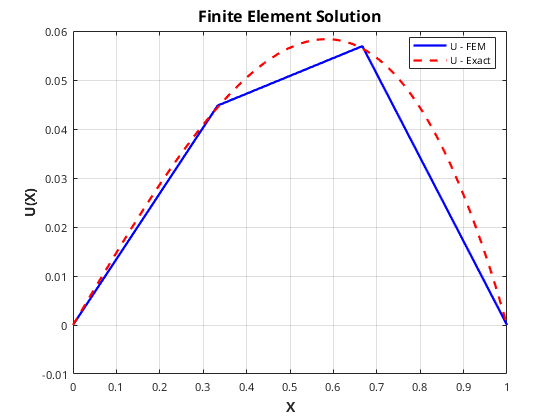
\includegraphics{lec34n-ex1-sol.png}
\caption{Approximate solution with three linear elements.}
\label{fig:lec34n-ex1-sol}
\end{marginfigure}
\begin{lstlisting}[style=myMatlab,name=lec34n-ex1]
% Gather into system matrix and vector
A = -K1 - K2;
RHS = -R;

% apply boundary conditions
A(1,:) = 0; A(1,1) = 1; RHS(1) = Ua;
A(nnodes,:) = 0; A(nnodes,nnodes) = 1; RHS(nnodes) = Ub;

% solve the system of equations
u = A\RHS;

%% Plot the solution and check error
x = gcoord;
x_gold = linspace(a,b,1000);
figure(1)
plot(x,u','-b',...
    x_gold,u_exact(x_gold),'--r',...
    'linewidth',2);
title('Finite Element Solution',...
    'FontSize',14,'FontWeight','bold');
xlabel('X','FontSize',12,'FontWeight','bold');
ylabel('U(X)','FontSize',12,'FontWeight','bold');
grid on
legend('U - FEM','U - Exact','Location','best');
\end{lstlisting}

Of course we would not normally just use three elements; if we increase the number of finite elements to 30, the solution is much improved.  This solution along with a plot of absolute error is shown in Figure \ref{fig:lec34n-ex1-sol-refined}.  If greater precision is needed, we can simply increase the number of elements.

\begin{marginfigure}[1.0cm]
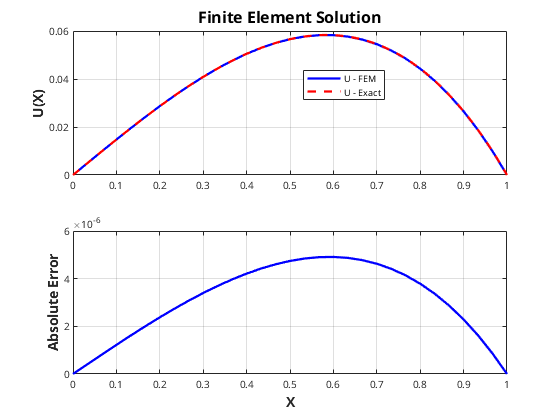
\includegraphics{lec34n-ex1-sol-refined.png}
\caption{FEM solution with 30 elements.}
\label{fig:lec34n-ex1-sol-refined}
\end{marginfigure}


\subsection{FEM with P-refinement}
So far we have not taken advantage of the generality of the FEM approach to finding approximate solutions to boundary value problems.  We have presented the mathematical analysis and an accompanying MATLAB script that solves one problem with FEM using linear shape functions on an arbitrary number of elements.  This allowed us to carry out h-refinement to improve our solution.  In the section we will slightly generalize the structure of the MATLAB code and incorporate the ability to increase the polynomial order of the shape functions used within each element.  A few notes before we begin to present the code:
\begin{enumerate}
\item The basic structure of the MATLAB implementation is the same.  The main difference is that the shape functions and the derivative of the shape functions will be created at ``run time'' based on input from the script.  

\item Higher order shape functions will mean that the calculations for populating the local arrays $K_1$, $K_2$ and $r$ will be more lengthy but, it turns out, that we will accomplish this task with \emph{less code} by generalizing the local element matrix calculation.
\end{enumerate}
Now for the code:
\setcounter{lstannotation}{0}
\marginnote{

\vspace{1.5cm}

\noindent\ref{lst:ann34n-ex2-1} Notice that we are, again, going to solve a problem that we've done before.  Here we will confirm that we get the same result that we did with the less generalized implementation.

\vspace{0.1cm}

\noindent\ref{lst:ann34n-ex2-2} This local function will be presented later but you should note right away that the \emph{outputs} from \lstinline[style=myMatlab]{genMesh1D}, the \lstinline[style=myMatlab]{gcoord} and \lstinline[style=myMatlab]{nodes} arrays fulfill the same purpose as they did in the previous code; provide the x-coordinate for all nodes and provide the local-to-global node number mapping for each element.  It is a good idea to establish standardized data structures when implementing FEM codes and this is intended to be an example of this type of standardization.

\vspace{0.1cm} 

\noindent\ref{lst:ann34n-ex2-3} As the function name suggests, we are going to get the sample points and weights for the requested Gauss quadrature scheme.  This is an alternative to hard-coding the sample points and weights like was done for the previous example.

}
\begin{lstlisting}[style=myMatlab,name=lec34n-ex2]
clear
clc
close 'all'

%% Exact Solution
u_exact = @(x) x - sinh(x)./sinh(1);

%% Finite Element Parameters and Data Structures
a = 0; b = 1;
Ua = 0; Ub = 0; % boundary conditions
nelem = 3; % select # of elements /*!\annotation{lst:ann34n-ex2-1}!*/
order = 1;

[gcoord,nodes] = genMesh1D(a,b,nelem,order); /*!\annotation{lst:ann34n-ex2-2}!*/

% nldofs = number of local dofs for each element
nldofs = order+1;

% global x-coordinate of each node
nnodes = length(gcoord);

% sample points for Gauss Quadrature
nqp = order+1; % number of sample points requested
[q,w] = getGPandWeights(nqp); /*!\annotation{lst:ann34n-ex2-3}!*/


% initialize global arrays
K1 = zeros(nnodes,nnodes);
K2 = zeros(nnodes,nnodes);
R = zeros(nnodes,1);
\end{lstlisting}
The next task will be to carry out the numeric integration and element assembly process.  Since we allow the user to specify the order of interpolation, we will need to generate appropriate shape functions and their derivatives.  Leveraging the work we did earlier in the course we will use Lagrange polynomials (Lecture 15) for the shape functions and the derivatives of those Lagrange polynomials (Lecture 18).
\marginnote{

\vspace{1.5cm}

\noindent\ref{lst:ann34n-ex2-4} These arrays are the same as in the last example except that they must be sized according to the number of local degrees of freedom, \lstinline[style=myMatlab]{nldofs}.  In the technical parlance, each unknown is often referred to as a ``degree of freedom.''

\vspace{2.75cm}

\noindent\ref{lst:ann34n-ex2-5} These local functions will be presented separately.

\vspace{1.75cm}

\noindent\ref{lst:ann34n-ex2-6} This is essentially the same as in the last example except that now loops are used so that the arbitrary number of local degrees of freedom can be handled seamlessly.

}
\begin{lstlisting}[style=myMatlab,name=lec34n-ex2]
% carry out assembly process
for ele = 1:nelem
    % local arrays to be populated
    k1 = zeros(nldofs,nldofs);  /*!\annotation{lst:ann34n-ex2-4}!*/
    k2 = zeros(nldofs,nldofs);
    r = zeros(nldofs,1);
    
    % local mapping for GQ
    aL = gcoord(nodes(ele,1));
    bL = gcoord(nodes(ele,nldofs));
    xT = @(t) ((bL - aL)*t + aL + bL)/2;
    Jac = (bL - aL)/2;

    % Get sample points for shape functions
    xgl = gcoord(nodes(ele,:));
    
    % get Lagrange Interpolant of requested order
    H = getLagrangeInterp(xgl);  /*!\annotation{lst:ann34n-ex2-5}!*/
    Hp = getLagrangeInterpDeriv(xgl);

    for qp = 1:nqp        
        % sum weighted contribution at Gauss Points
        for i = 1:nldofs
            for j = 1:nldofs
                k1(i,j) = k1(i,j) + ...
                    Hp{i}(xT(q(qp)))*Hp{j}(xT(q(qp)))*w(qp); /*!\annotation{lst:ann34n-ex2-6}!*/
                k2(i,j) = k2(i,j) + ...
                    H{i}(xT(q(qp)))*H{j}(xT(q(qp)))*w(qp);
            end % j
            r(i) = r(i) + xT(q(qp))*H{i}(xT(q(qp)))*w(qp);
        end % i     
    end % qp
    % apply Jacobian to map to physical coordinates
    k1 = k1*Jac; k2 = k2*Jac; r = r*Jac;

    % add local arrays to global arrays "assembly"
    for i = 1:nldofs
        for j = 1:nldofs
            row = nodes(ele,i); col = nodes(ele,j);
            K1(row,col) = K1(row,col) + k1(i,j);
            K2(row,col) = K2(row,col) + k2(i,j);
        end % j
        dof = nodes(ele,i);
        R(dof) = R(dof) + r(i);
    end % i
end % numel

% apply boundary conditions
A = -K1 - K2;
RHS = -R;
A(1,:) = 0; A(1,1) = 1; RHS(1) = Ua;
A(nnodes,:) = 0; A(nnodes,nnodes) = 1; RHS(nnodes) = Ub;

% solve the system of equations
u = A\RHS;
\end{lstlisting}
\begin{marginfigure}[-3.0cm]
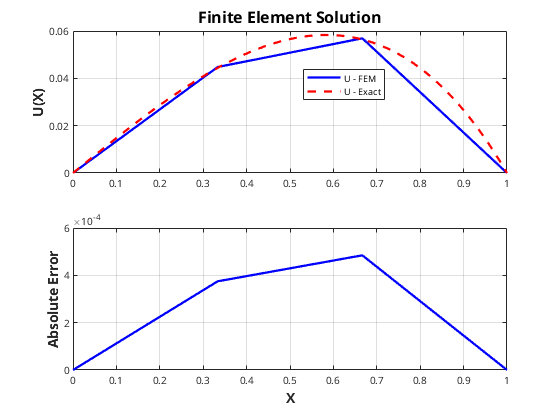
\includegraphics{lec34n-ex2-sol-1-3.png}
\caption{FEM Solution for 3 linear elements, revisited.}
\label{fig:lec34n-ex2-sol-1-3}
\end{marginfigure}

\begin{marginfigure}[1.0cm]
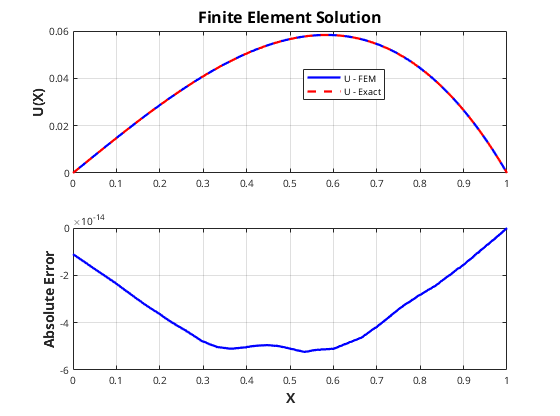
\includegraphics{lec34n-ex2-sol-9-3.png}
\caption{FEM Solution for 3 elements with 9\textsuperscript{th}-order shape functions.}
\label{fig:lec34n-ex2-sol-9-3}
\end{marginfigure}
Some solutions are shown in Figure \ref{fig:lec34n-ex2-sol-1-3} and Figure \ref{fig:lec34n-ex2-sol-9-3}.  This shows the benefit of p-refinement. Similar precision can be obtained with lower-order shape functions if the number of elements is increased, in hp-refinement. 

\subsection{Local Functions}
The several local functions that were used for the generalized MATLAB implementation are shown in this section.

\vspace{0.25cm}

\noindent\textbf{genMesh1D}
\begin{lstlisting}[style=myMatlab,name=lec34n-ex2]
function [gcoord,nodes] = genMesh1D(a,b,nelem,order)
%generates the global coordinates of all mesh points and 
%provides a mapping between global node number and local
%element dof for all elements.

ldofs = order + 1; % need order+1 local degrees of freedom

ndofs = nelem+1 + (ldofs-2)*nelem;
gcoord = nan(1,ndofs);
nodes = nan(nelem,ldofs);
ele_boundaries = linspace(a,b,nelem+1);
dof_it = 1;
for e = 1:nelem 
    aL = ele_boundaries(e);
    bL = ele_boundaries(e+1);
    xT = @(t) ((bL - aL)*t + aL + bL)/2;
    [xgl,~]=legendre_gauss_lobatto(ldofs);
    xgl = xT(xgl); % translate to current element

    for ld = 1:ldofs
        nodes(e,ld) = dof_it;
        gcoord(dof_it) = xgl(ld);
        dof_it = dof_it + 1;
    end % ld
    % set back for shared node at element boundary
    dof_it = dof_it - 1; 
end % e

end
\end{lstlisting}

\vspace{0.25cm}

\noindent\textbf{getGPandWeights}
This function, as the name indicates, gets the Gauss points and weights for the specified number of points.  This function implements the theory described in Lecture 20 for Gauss quadrature.  

\vspace{0.1cm}


\begin{lstlisting}[style=myMatlab,name=lec34n-ex2]
function [xgl, wgl] = getGPandWeights(P)
%GetGP(P) Get Gauss Points and Weights for P-point Gauss Quad
%   input:  P - # of Gauss Points to use in integration
%  output:  xgl - vector of gauss points
%           wgl - vector of weights
%
%
%% Generate Legendre Polynomials of Order 0 through P
% Store handles to these functions in a cell array.
isQuadSet = false; % flag for special exit of quadrature scheme.
Pn = cell(P+1,1);
Pn{1} = @(x) 1;
Pn{2} = @(x) x;
if P == 0
    error('P must be greater than 0');
elseif P == 1
    xgl = 0; % for P == 1, GQ reduces to midpoint rule 
    wgl = 2;
    isQuadSet = true;
else
    for n = 2:P
        % use recurrence relation to generate higher order 
        % Legendre Polynomials ("Pn functions")
        Pn{n+1} = @(x) ...
            (2*(n-1)+1)*x.*Pn{n}(x)./((n-1)+1)...
            - (n-1)*Pn{n-1}(x)./((n-1)+1);
    end
end

if ~(isQuadSet)
    %% Compute Roots to the Pth order Legendre Polynomial
    
    % get an approximate zeros from the Chebychev points
    Tch = @(n) cos(((2*(1:n)) - 1)*pi./(2*n));
    xEst = Tch(P);
    
    % use fzero and approximate root to find root of the Pn polynomial.
    xgl = NaN(1,P);
    for r = 1:P
        xgl(r) = fzero(Pn{P+1},xEst(r));
    end
    
    %% Sample Pn functions at roots of Pth order function
    % These values form the matrix that will be used to 
    % find the weights forthe quadrature method.
    if P == 1
        A = xgl(1);
    else
        A = NaN(P,P);
        A(1,:) = Pn{1}(xgl);
        A(2,:) = Pn{2}(xgl);
        for n = 2:(P-1)
            A((n+1),:) = Pn{n+1}(xgl);
        end
    end
    
    %% Form LHS vector
    % These are equal to the integral of the lower order Pn 
    % functions over the domain.  For P0, the integral 
    % equals 2; for all other orders, the integral is zero.
    k = zeros(P,1); k(1) = 2;
    
    %% Solve for the weights
    wgl = A\k;
end
end
\end{lstlisting}

\vspace{0.5cm}

\noindent\textbf{genLagrangeInterp}

\begin{lstlisting}[style=myMatlab,name=lec34n-ex2]
function H = getLagrangeInterp(Xi)
%function dH = getLagrangeInterp(Xi)
% input Xi - vector of sample points
% output H - cell array containing Lagrange Interp Functions

n = length(Xi);
H = cell(n,1);

for i = 1:n
    L = @(x) 1; %<-- initialize the Lagrange Function
    for j = 1:n
        if j ~= i
            L = @(x) L(x).*((x - Xi(j))./(Xi(i) - Xi(j)));
        end
    end
    H{i} = L;
end
end
\end{lstlisting}

\vspace{0.5cm}

\noindent\textbf{genLagrangeInterpDeriv}

\begin{lstlisting}[style=myMatlab,name=lec34n-ex2]
function dH = getLagrangeInterpDeriv(Xi)
%function dH = getLagrangeInterpDerive(Xi)
% input: Xi - vector of sample points
% output dH - cell array containing the derivative 
% of Lagrange Interpolant functions.
n = length(Xi);
dH = cell(n,1);

for i = 1:n
    dLi = @(x) 0;
    for k = 1:n
        if k ~= i
            dLp = @(x) 1;
            for j = 1:n
                if ((j ~= i) && (j ~= k))
                    dLp = @(x) dLp(x).*...
                        (x - Xi(j))./(Xi(i) - Xi(j));
                end
            end
            dLi = @(x) dLi(x) + ...
                (1./(Xi(i) - Xi(k))).*dLp(x);
        end
        
    end
    dH{i} = dLi;
end
end
\end{lstlisting}

\vspace{3.5cm}

\noindent\textbf{legendre\_poly}

\begin{lstlisting}[style=myMatlab,name=lec34n-ex2]
function [L0,L0_1,L0_2] = legendre_poly(p,x)
%-------------------------------------------------------%
%This code computes the Legendre Polynomials and 
%its 1st and 2nd derivatives
%Written by F.X. Giraldo on 4/2008
%           Department of Applied Mathematics
%           Naval Postgraduate School 
%           Monterey, CA 93943-5216
%-------------------------------------------------------%
L1=0;L1_1=0;L1_2=0;
L0=1;L0_1=0;L0_2=0;

for i=1:p
   L2=L1;L2_1=L1_1;L2_2=L1_2;
   L1=L0;L1_1=L0_1;L1_2=L0_2;
   a=(2*i-1)/i;
   b=(i-1)/i;
   L0=a*x*L1 - b*L2;
   L0_1=a*(L1 + x*L1_1) - b*L2_1;
   L0_2=a*(2*L1_1 + x*L1_2) - b*L2_2;
end
end
\end{lstlisting}

\vspace{0.5cm}

\noindent\textbf{legendre\_gauss\_lobatto}

\begin{lstlisting}[style=myMatlab,name=lec34n-ex2]
function [xgl,wgl] = legendre_gauss_lobatto(P)
%------------------------------------------------------------%
%This code computes the Legendre-Gauss-Lobatto points 
%and weights which are the roots of the Lobatto Polynomials.
%Written by F.X. Giraldo on 4/2008
%           Department of Applied Mathematics
%           Naval Postgraduate School 
%           Monterey, CA 93943-5216
%------------------------------------------------------------%

p=P-1; %Order of the Polynomials
ph=floor( (p+1)/2 );
xgl = nan(1,P);
wgl = nan(1,P);
for i=1:ph
   % estimate the roots
   x=cos( (2*i-1)*pi/(2*p+1) );
   for k=1:20
      % evaluate L, dL, ddL
      [L0,L0_1,L0_2]=legendre_poly(p,x); 
      %Compute Nth order Derivatives of Legendre Polys
      
      %Get new Newton Iteration
      dx=-(1-x^2)*L0_1/(-2*x*L0_1 + (1-x^2)*L0_2);
      x=x+dx;
      if (abs(dx) < 1.0e-20) 
         break
      end
   end
   xgl(p+2-i)=x;
   wgl(p+2-i)=2/(p*(p+1)*L0^2);
end

%Check for Zero Root
if (p+1 ~= 2*ph)
   x=0;
   [L0,~,~]=legendre_poly(p,x);
   xgl(ph+1)=x;
   wgl(ph+1)=2/(p*(p+1)*L0^2);
end
   
%Find remainder of roots via symmetry
for i=1:ph
   xgl(i)=-xgl(p+2-i);
   wgl(i)=+wgl(p+2-i);
end   
end
\end{lstlisting}
